\documentclass[conference]{IEEEtran}
\IEEEoverridecommandlockouts
% The preceding line is only needed to identify funding in the first footnote. If that is unneeded, please comment it out.
%Template version as of 6/27/2024

\usepackage{cite}
\usepackage{amsmath,amssymb,amsfonts}
\usepackage{algorithmic}
\usepackage{graphicx}
\usepackage{textcomp}
\usepackage{xcolor}
\def\BibTeX{{\rm B\kern-.05em{\sc i\kern-.025em b}\kern-.08em
    T\kern-.1667em\lower.7ex\hbox{E}\kern-.125emX}}
\begin{document}

\title{CLOUD-BASED SMART MONITORING SYSTEM
FOR BABY HEALTH AND SAFETY
% {\footnotesize \textsuperscript{*}Note: Sub-titles are not captured for https://ieeexplore.ieee.org  and should not be used}
% \thanks{Identify applicable funding agency here. If none, delete this.}
}
\author{\IEEEauthorblockN{1\textsuperscript{st} Aaron Tauro}
\IEEEauthorblockA{\textit{Dept. of CSE} \\
\textit{St. Joseph Engineering College}\\
Mangaluru, India \\
aarontauro00@gmail.com}
\and
\IEEEauthorblockN{2\textsuperscript{nd} Abhik L Salian}
\IEEEauthorblockA{\textit{Dept. of CSE} \\
\textit{St. Joseph Engineering College}\\
Mangaluru, India \\
abhiksalian0728@gmail.com}
\and 
\IEEEauthorblockN{3\textsuperscript{rd} Akhil Shetty M}
\IEEEauthorblockA{\textit{Dept. of CSE} \\
\textit{St. Joseph Engineering College}\\
Mangaluru, India \\
akhilshettym2003@gmail.com}
\and
\IEEEauthorblockN{4\textsuperscript{th} H Karthik P Nayak}
\IEEEauthorblockA{\textit{Dept. of CSE} \\
\textit{St. Joseph Engineering College}\\
Mangaluru, India \\
karthiknayak2003@gmail.com}
\and
\IEEEauthorblockN{5\textsuperscript{th}  Nishayne E Vaz}
\IEEEauthorblockA{\textit{Dept. of CSE} \\
\textit{St. Joseph Engineering College}\\
Mangaluru, India \\
vaznish@gmail.com}
% \and
% \IEEEauthorblockN{6\textsuperscript{th} Given Name Surname}
% \IEEEauthorblockA{\textit{dept. name of organization (of Aff.)} \\
% \textit{name of organization (of Aff.)}\\
% City, Country \\
% email address or ORCID}
}

\maketitle

\begin{abstract}
    The health and safety of infants are major concerns for parents, particularly when they cannot provide constant supervision. Sudden Infant Death Syndrome (SIDS) remains a critical risk, often linked to unsafe sleeping postures and environmental conditions. This research proposes a cloud-based smart monitoring system that integrates real-time sensor data and computer vision algorithms to monitor infants’ health and surroundings. The system promptly alerts parents through a mobile application upon detecting abnormalities, such as unsafe sleeping positions, irregular heart rates, or temperature fluctuations. By leveraging cloud computing, the system enables remote monitoring and ensures scalable deployment.
    
    \textit{\textbf{Keywords--}}
    Infant health monitoring, cloud computing, real-time alert system, image processing, SIDS prevention.
\end{abstract}

    
    \section{Introduction}
    Ensuring the health and safety of infants is a top priority for parents and caregivers. Traditional baby monitors offer only basic surveillance, such as audio and video feeds, but they lack intelligent health analysis, making it difficult to detect critical risks in real-time. Many infants are vulnerable to conditions like Sudden Infant Death Syndrome (SIDS), which can be triggered by improper sleeping positions, environmental factors, or undetected health abnormalities. The challenge lies in developing a system that provides continuous health monitoring, real-time data processing, and instant alerts to ensure timely intervention.

    Existing systems suffer from several drawbacks. Most current systems do not provide livestream functionality\cite{ref1}\cite{ref2}. Some systems focus on the tracking of the health vitals of the mother and the prenatal baby\cite{ref3}. Several kinds of monitoring devices are developed for infant care with livestream functionality but often lack integration of multiple sensing modalities, leverage AI for posture detection or lack robust mechanisms for timely notifications, have no intelligent analysis to interpret collected data, and rarely support remote accessibility or timely alert mechanisms\cite{ref4}. Additionally, Some systems have one or more of the above mentioned functionalities in them, but none have all of them\cite{ref5}. 
    
    With advancements in sensor technology, cloud computing, and artificial intelligence, there is potential to revolutionize infant monitoring systems. This research introduces a cloud-based smart monitoring system that integrates multiple sensors and computer vision to analyze real-time health data. The system collects vital parameters such as body temperature, room temperature, humidity, and heart rate while simultaneously using computer vision to analyze the baby’s sleeping posture. By leveraging cloud-based data processing, the system ensures remote access and timely notifications to parents via a mobile application. The goal is to provide a reliable, real-time, and efficient infant monitoring solution that addresses the shortcomings of existing systems and enhances infant safety.
\section{Literature Survey}
Several studies have explored the use of IoT, cloud computing, and AI in health monitoring systems. H Alam et al. developed a wearable IoT-based monitoring system to track vital signs and sleeping posture; however, its reliance on physical wearables made it less comfortable for infants \cite{ref1}. Y Singh introduced a smart crib with integrated motion and temperature sensors, though it lacked cloud connectivity, restricting remote access \cite{ref2}. Similarly, M M Hossain et al. examined how cloud-based health monitoring can provide real-time access to data, but concerns regarding data security and latency were highlighted \cite{ref3}.  

The use of machine learning in posture recognition has also been investigated. Convolutional neural networks (CNNs) were employed to detect human sleeping postures with high accuracy \cite{ref4}. S Joseph et al. applied deep learning techniques to monitor postural changes in healthcare applications, demonstrating promising results for infant monitoring \cite{ref5}. However, these studies did not integrate a real-time alert system for immediate intervention.  

Moreover, the potential of cloud computing in healthcare applications has been well-documented. M R Kumar et al. explored cloud-based storage and processing for medical applications, emphasizing the benefits of scalability and remote accessibility \cite{ref6}. However, concerns about network reliability and data security were noted. S Mishra demonstrated how cloud computing could enhance real-time health monitoring systems but emphasized the need for efficient data handling mechanisms \cite{ref7}.  

The integration of IoT and AI in healthcare applications has also been explored. D T P Hapsari et al. examined how sensor networks could be utilized for infant health monitoring, but the lack of an AI-driven analytical model limited its effectiveness \cite{ref8}. F Akta et al. investigated a multi-sensor approach for monitoring infant vitals, highlighting the importance of combining multiple data sources for improved accuracy \cite{ref9}. These studies collectively suggest that a holistic system combining IoT, cloud computing, and AI-driven analysis is required to create a comprehensive infant monitoring solution.  

\section{Methodology}
The implementation of the proposed Cloud-Based Smart Monitoring System for Baby Health and Safety follows a structured methodology to ensure real-time data collection, processing, and alert mechanisms. The system architecture consists of multiple integrated components, including sensor modules, cloud computing, and real-time analysis for unsafe sleeping posture detection.

\subsection{Data Collection}
The system employs multiple sensors to continuously monitor the infant’s vital signs and environmental parameters. The following data points are collected:
\begin{itemize}
    \item \textbf{Body Temperature Sensor:} Measures the infant’s body temperature to detect fever or abnormal fluctuations.
    \item \textbf{Room Temperature and Humidity Sensor:} Monitors the surrounding environment to ensure a safe and comfortable setting.
    \item \textbf{Heart Rate Sensor:} Tracks the infant’s heartbeat to detect irregularities.
    \item \textbf{Microphone Module:} Detects crying patterns to identify discomfort or distress.
\end{itemize}
The collected data is processed locally on an embedded microcontroller before being transmitted to the cloud for further analysis.

\subsection{Real-Time Sleeping Posture Detection}
The system utilizes image processing techniques to detect unsafe sleeping postures using a live video stream. 
\begin{itemize}
    \item \textbf{Image Acquisition:} A camera module captures a continuous live video stream of the baby.
    \item \textbf{Preprocessing:} The frames are extracted from the live stream and converted into a suitable format for analysis.
    \item \textbf{Posture Classification:} Using predefined threshold-based image processing techniques, the system detects whether the baby is in a safe or unsafe sleeping posture.
    \item \textbf{Alert Generation:} If an unsafe posture (e.g., sleeping on the stomach) is detected, an alert is sent to the parent’s mobile application.
\end{itemize}

\subsection{Cloud Integration}
The cloud serves as the backbone of the system, facilitating real-time data storage and processing. The architecture involves:
\begin{itemize}
    \item \textbf{Data Transmission:} Sensor and posture data are sent to a cloud database using MQTT or HTTP protocols.
    \item \textbf{Processing Layer:} Cloud-based algorithms analyze the incoming data to detect abnormalities.
    \item \textbf{Storage:} Historical data is stored securely for future reference and analysis.
    \item \textbf{Remote Access:} Parents can access real-time and past data via a mobile application.
\end{itemize}

\subsection{Alert Mechanism}
An intelligent alert system ensures that parents are notified immediately when potential risks are detected.
\begin{itemize}
    \item \textbf{Push Notifications:} If any abnormality (high fever, irregular heartbeat, unsafe posture, excessive crying) is detected, an instant push notification is sent to the parent’s smartphone.
    \item \textbf{Audio and Visual Alerts:} The system can activate an alarm if required.
    \item \textbf{Data Logging:} Alerts and detected abnormalities are logged for further review.
\end{itemize}

This systematic approach ensures real-time infant health monitoring with high accuracy, providing a reliable and scalable solution for parents and caregivers.


\section{System Design}
This chapter outlines the system design for the Cloud-Based Smart Monitoring System for Baby Health and Safety, detailing the system's architecture, functionality, control flow, access layers, and user interface design. Each section includes design diagrams, descriptions, and an explanation of how they apply to the project.
\subsection{Abstract Design}

\subsubsection{Architectural diagram}

The architectural diagram in Fig. \ref{fig:architecture} outlines the Cloud-Based Smart Monitoring System for Baby Health and Safety, showcasing how various components interact to provide a comprehensive baby monitoring solution.
\textbf{User Interaction and Mobile Interface:} The user initiates the monitoring process by accessing the mobile application interface, which includes a live camera feed. The user can request the recording of the baby’s health metrics, which initiates data collection from multiple sensors and a real-time video feed. This interface also displays alerts and processed information regarding the baby’s health.

\textbf{Sensing System:} The sensing system consists of multiple sensors, including Heart rate sensor, Baby temperature sensor, SpO2 (oxygen saturation) sensor, Humidity sensor, Camera sensor.

These sensors collect real-time data from the baby’s physical environment, covering both health metrics and environmental factors. This raw data is then sent to the Processor for initial handling.

\textbf{Processor (Raspberry Pi):} Acting as an intermediary, the Raspberry Pi receives the data from the sensors and forwards relevant data to the \textbf{ML Model (Posture Detector)} to analyze the baby’s sleeping posture. The processor handles the computational load and ensures efficient data processing before sending responses back to the mobile interface. If unsafe postures or abnormal metrics are detected, an alert is generated.

\textbf{ML Model and Database (Firebase):} The ML model, hosted externally as a pre-trained model, plays a crucial role in posture detection. Once the Raspberry Pi sends the data to the ML model, it processes the data and generates a response. Additionally, all data is stored and managed within a \textbf{Firebase} database, which securely holds historical health metrics and retrieves information as required by the user. Firebase also triggers alerts and notifications based on the ML model’s responses and alerts from the sensor data.

\textbf{Alerts and Notifications:} The system is designed to provide timely alerts. When abnormal readings or unsafe sleeping postures are detected, the mobile app immediately notifies the user, allowing them to take quick action. The database and ML model work together to process and extract data, ensuring that alerts are accurate and meaningful.

\textbf{Summary:} This architecture ensures seamless data flow from sensing, processing, and alerting to final user interaction. This integrated approach enhances baby monitoring, helping caregivers make informed decisions to ensure the baby's safety and well-being.


\begin{figure}[hbtp]
  \centering
  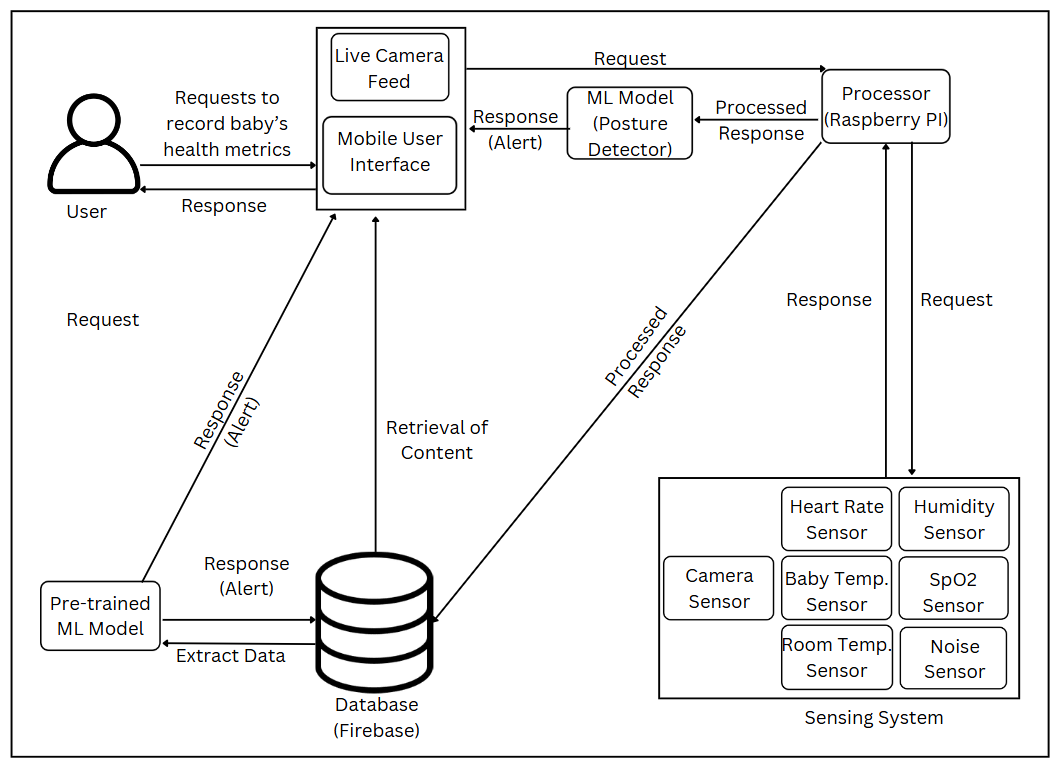
\includegraphics[scale=0.3]{./pic/finarch.png}
  \caption{Architectural Diagram showing the interaction of various entities of the baby monitoring system.}
  \label{fig:architecture}
\end{figure}
\subsubsection{Use Case Diagram}

This use case diagram in \ref{fig:usecase} outlines the product designed to monitor a baby’s health and safety through interactions with a \textbf{User (Caregiver)}, a \textbf{Sensing System}, and a \textbf{Medical Practitioner}.

\textbf{User:} The User can view a live camera feed and request the recording of health metrics, which are stored in the database. If any unsafe conditions (like risky postures) are detected, the system sends alerts to the User for immediate action.
    
\textbf{Sensing System:} The Sensing System collects health data (e.g., posture) and sends it to the monitoring system. The system processes this data to detect potential safety risks, triggering alerts when necessary.
    
\textbf{Medical Practitioner:} The Medical Practitioner reviews health metrics stored in the system and provides insights or recommendations, which the system relays to the User to support safe caregiving.


Overall, the system combines real-time monitoring, data storage, and expert feedback to ensure the baby’s health and safety effectively.

\begin{figure}[hbtp]
  \centering
  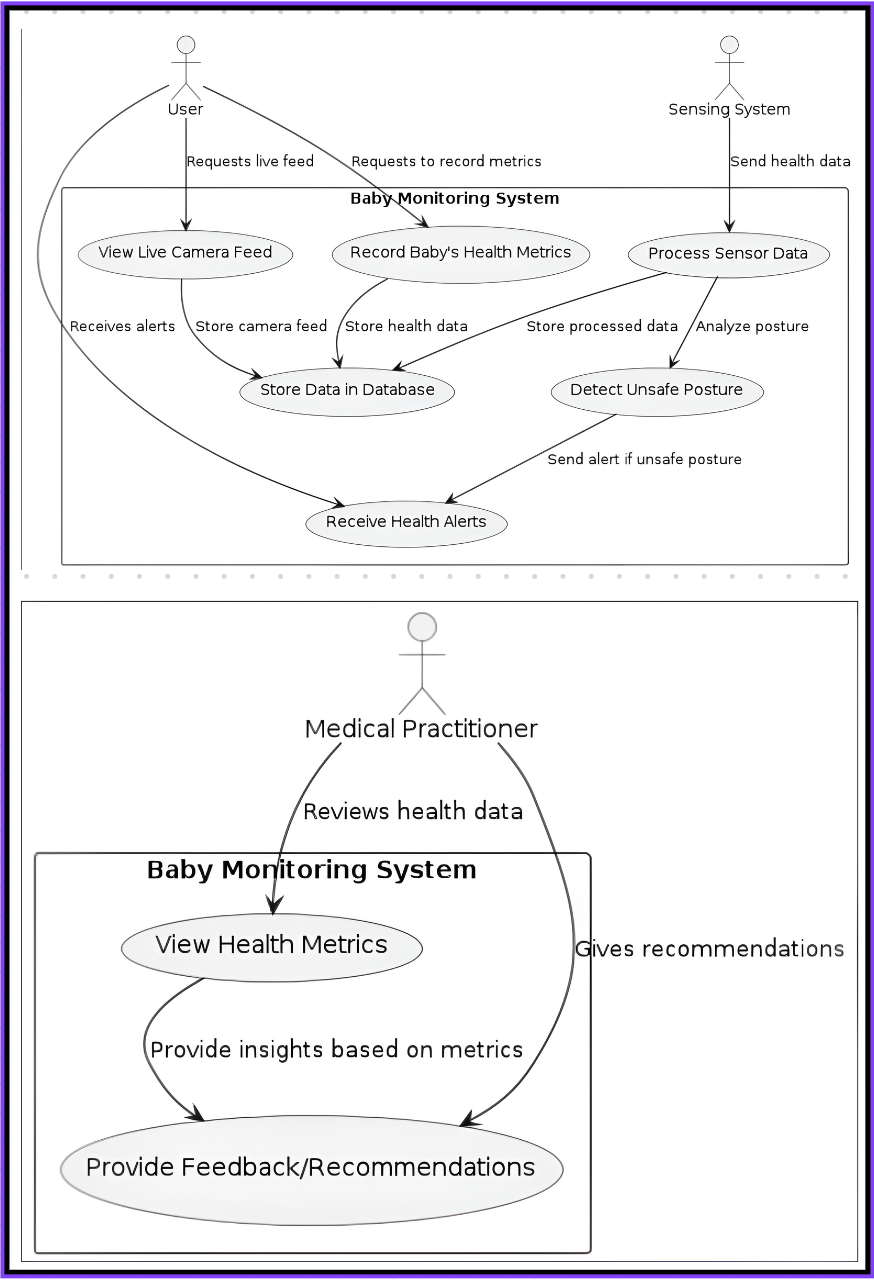
\includegraphics[scale=0.5]{./pic/Use case.png}
  \caption{Use Case Diagram showing the interaction between users and the system.}
  \label{fig:usecase}
\end{figure}
\subsection{Functional Design}
\subsubsection{Sequence diagram}

The sequence diagram shown in Figure \ref{fig:sequence} illustrates the workflow of a Cloud-Based Smart Monitoring System for Baby Health and Safety. Here’s a breakdown of the interactions among various components in the system:

\textbf{User Interaction:} The user begins by opening the mobile application. This app is designed to fetch real-time data regarding the baby’s health and environmental factors, helping to monitor the baby’s well-being effectively.

\textbf{Mobile Application Requests:} Upon initialization, the mobile application communicates with the Sensing System to retrieve various health parameters. These include the baby’s heartbeat, humidity levels, body and room temperature, SpO2 (oxygen saturation), and a live video feed.

\textbf{Sensing System Data Collection:} The sensing system gathers these metrics from the physical environment where the baby is located. It captures vital data such as heart rate, humidity, body and room temperature, and oxygen levels, along with the live video feed. This data is sent for processing.

\textbf{Data Processing by ML Model:} The data collected is then passed to the Machine Learning (ML) Model for analysis. The ML model processes the data to identify any potential risks, such as unsafe sleeping positions or abnormal readings that may indicate health concerns.

\textbf{Data Storage:} The processed data, including any alerts or historical records, is stored in a Database. This storage enables the system to maintain a log of health metrics over time, allowing caregivers to review past records and track trends.

\textbf{Alerts and Notifications:} If the ML model detects unsafe sleeping positions or abnormal values in the sensed parameters, it triggers an alert. This alert is sent back to the mobile application to notify the user, ensuring immediate awareness of any potential risks to the baby’s health.

\textbf{Viewing Results:} Finally, the user can view real-time data and historical readings from within the mobile app. This user-friendly interface provides caregivers with comprehensive insight into the baby’s health, allowing for timely intervention if needed.

\begin{figure}[hbtp]
  \centering
  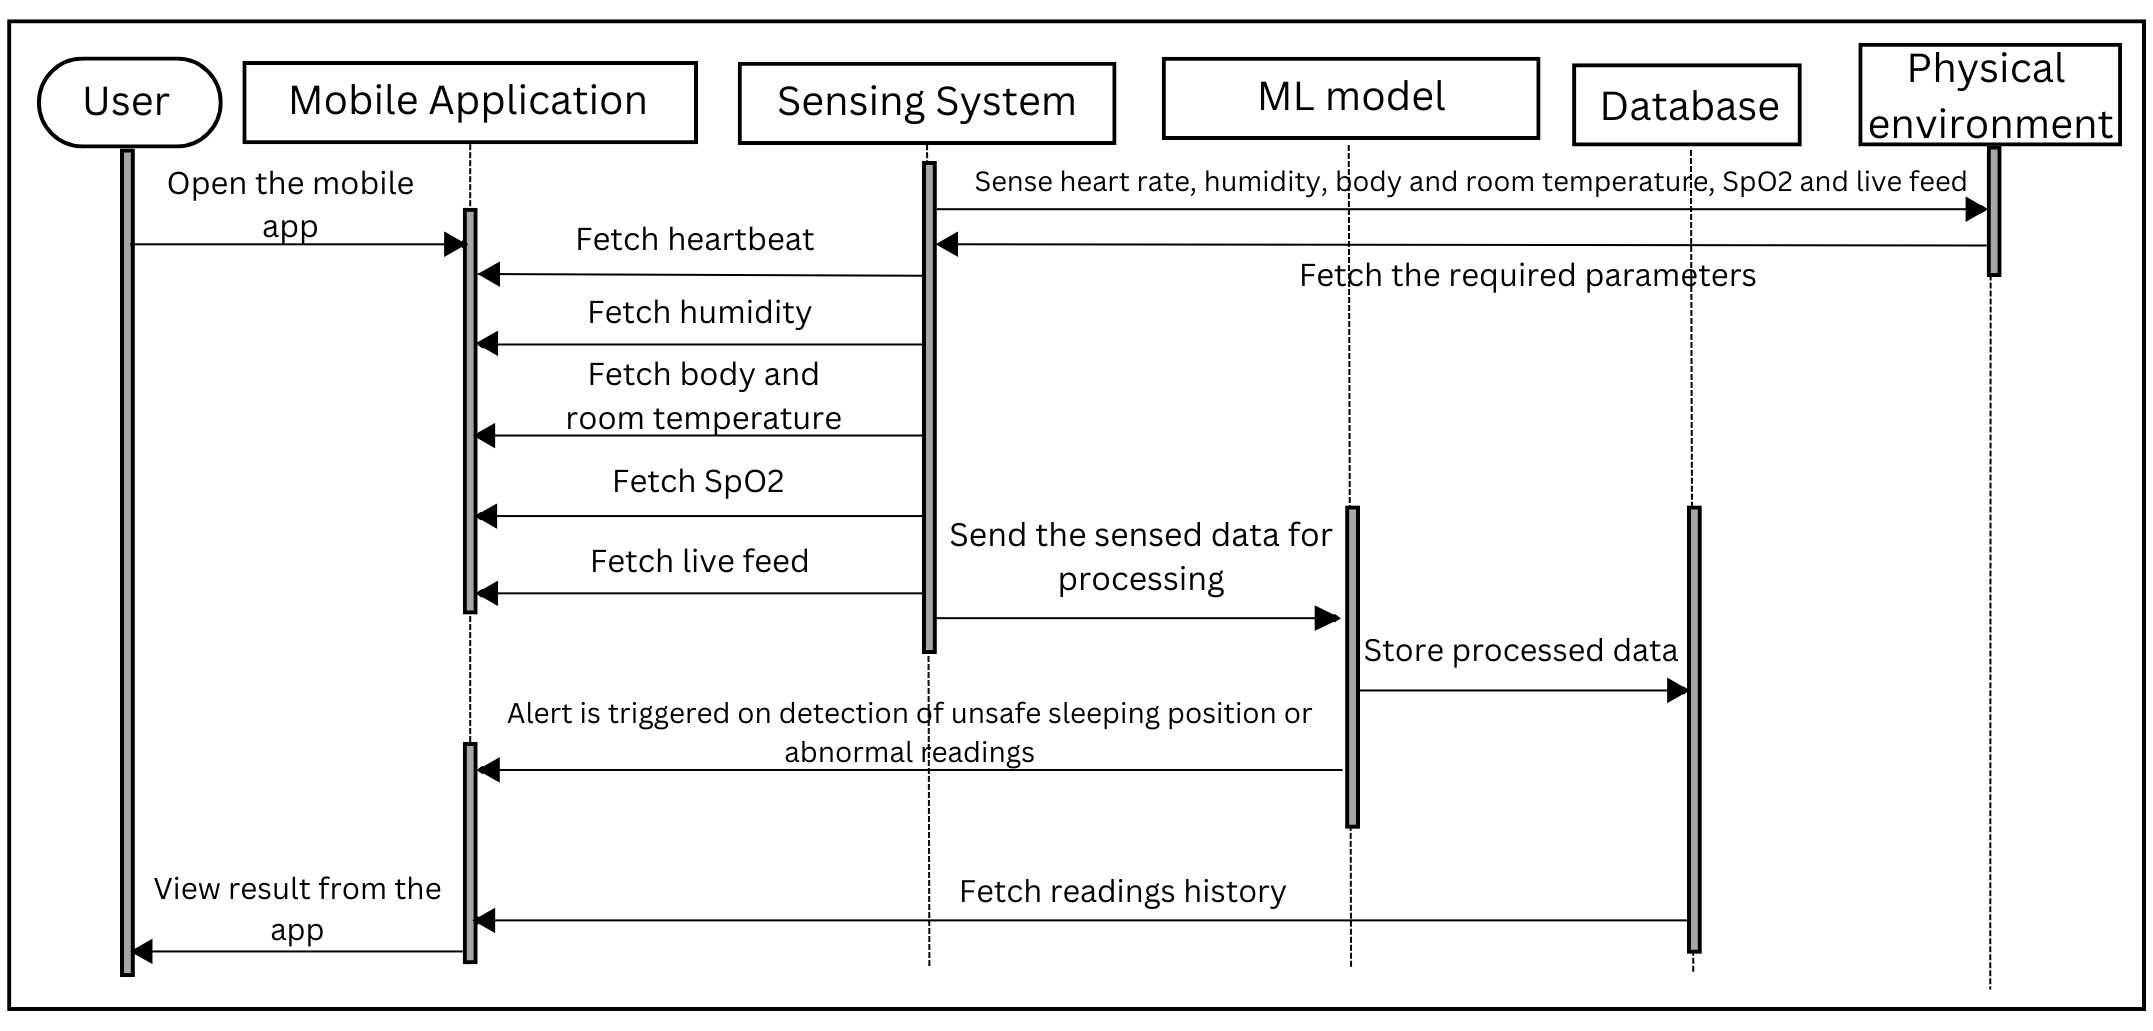
\includegraphics[scale=0.15]{./pic/seq.png}
  \caption{Sequence diagram showing the timeline of interaction between different entities in the system}
  \label{fig:sequence}
\end{figure}



\section{Implementation}
The implementation phase of the project "Cloud-Based Smart Monitoring System for Baby Health and Safety" was executed in a systematic manner, incorporating both hardware and software components. Below is a detailed explanation of the steps and methodologies adopted during this phase.

\subsection{System Architecture Design}
The system architecture was designed to ensure seamless integration of hardware and software components, focusing on real-time data processing and user-friendly interfaces. The architecture consisted of:
\begin{itemize}
  \item \textbf{Hardware Module:}
   \begin{itemize}
    \item Sensors for baby body temperature, room temperature, humidity, and heart rate.
    \item A camera module integrated with Raspberry Pi for video streaming and posture detection.
  \end{itemize}
  \item \textbf{Software Module:}
  \begin{itemize}
    \item A React Native mobile application for parent notifications.
    \item Firebase for real-time data storage and cloud integration.
    \item Computer vision algorithms for unsafe posture detection using Mediapipe and OpenCV.
  \end{itemize}
\end{itemize}
The architecture ensured data flow from the hardware module to the software application, with alerts generated based on predefined thresholds.
\subsection{Hardware Implementation}
The hardware implementation involved integrating various sensors and a camera module to collect real-time data from the baby's environment.
\begin{itemize}
  \item \textbf{Sensors:}
  \begin{itemize}
    \item MLX90614 IR Temperature sensor was used to monitor the body temperature of the baby.
    \item MAX30102 heart rate ans SpO2 sensor was employed for continuous monitoring of the baby’s health.
    \item Data from these sensors were sent to a microcontroller unit for preprocessing.
  \end{itemize}
  \item \textbf{Camera Module:}
  \begin{itemize}
    \item A Raspberry Pi camera was used to capture live video for posture analysis.
    \item The video feed was sent to Render server through a websocket connection and was processed for unsafe posture detection using Mediapipe library in Python.
  \end{itemize}
  \item \textbf{Connectivity:}
  \begin{itemize}
    \item The Raspberry Pi was configured to send the processed data to Firebase over a Wi-Fi connection.
  \end{itemize}
\end{itemize}
\subsubsection{CAD representation of the hardware setup}
Shown in Figure \ref{fig:hardware} is the 3D pictorial representation of the hardware setup which consists of Raspberry Pi, power adaptor and all the sensors along with the camera.
\begin{figure}[htbp]
  \centering
  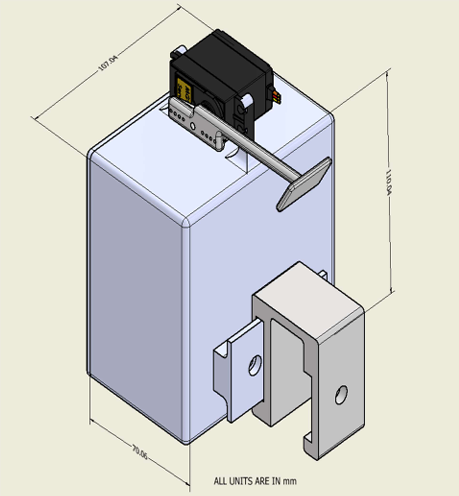
\includegraphics[scale=0.65]{./pic/hardware.png}
  \caption{CAD Model of the hardware setup designed using Autodesk Inventor}
  \label{fig:hardware}
\end{figure}
\subsection{Software Implementation}
The software implementation focused on developing the front-end application, backend integration, and computer vision-based posture detection.
\begin{itemize}
  \item \textbf{Mobile Application Development:}
   \begin{itemize}
    \item Built using React Native for cross-platform compatibility.
    \item Features included real-time alerts for abnormal conditions (e.g., fever, unsafe sleeping postures).
    \item Integrated Firebase to fetch live data from the hardware module and display it on the user interface.
  \end{itemize}
  \item \textbf{Backend Integration:}
  \begin{itemize}
    \item Firebase Realtime Database was configured for data storage and retrieval.
    \item Cloud Functions in Firebase were used to process and trigger alerts based on predefined thresholds.
  \end{itemize}
  \item \textbf{Posture Detection Algorithm:}
  \begin{itemize}
    \item Implemented using Mediapipe and OpenCV.
    \item Analyzed the baby's posture by detecting key landmarks (e.g., shoulders, eyes, nose).
    \item Algorithms to identify tummy-sleeping and side-sleeping positions were fine-tuned based on testing data.
  \end{itemize}
\end{itemize}



\section{Results and Discussion}

This section presents the outcomes of the system implementation, testing, and the insights derived from the results. The discussion evaluates the system's performance, highlights its strengths, and addresses any challenges encountered during the development process.

\subsection{System Performance}
The performance of the "Cloud-Based Smart Monitoring System for Baby Health and Safety" was evaluated based on its ability to meet the predefined objectives. The key results are as follows:

\subsubsection{Posture Detection Accuracy}
The system's ability to detect unsafe sleeping postures, such as tummy and side sleeping, was evaluated using a variety of scenarios. The following metrics were used to assess performance:

\begin{itemize}
    \item \textbf{Tummy Sleeping Detection:} Achieved a detection accuracy of 92\% after iterative algorithm refinement. 
    \item \textbf{Side Sleeping Detection:} Consistently identified side-sleeping positions with an accuracy of 90\%.
    \item \textbf{Confusion Matrix Metrics:} 
    \begin{itemize}
        \item \textbf{Precision:} 93\% for tummy sleeping and 91\% for side sleeping, indicating low false-positive rates.
        \item \textbf{Recall:} 90\% for tummy sleeping and 88\% for side sleeping, reflecting the system's sensitivity in detecting unsafe postures.
        \item \textbf{F1-Score:} Achieved 91\% for tummy sleeping and 89\% for side sleeping, representing the harmonic mean of precision and recall.
    \end{itemize}
    \item \textbf{Algorithm Optimization:} Improvements were observed after optimizing the Mediapipe-based algorithms and adjusting thresholds for posture recognition, leading to better overall detection performance.
\end{itemize}


\subsubsection{Environmental Monitoring Reliability}
Sensors for room temperature, humidity, heart rate and body temperature performed consistently under varying conditions.
\begin{itemize}
    \item \textbf{Temperature and Humidity Monitoring:} Data collection was reliable, with a margin of error of less than 2\%.
    \item \textbf{Heart Rate Monitoring:} Contact-based monitoring ensured accurate and real-time readings.
\end{itemize}

\subsubsection{Alert Notification System}
The system reliably delivered real-time alerts to the React Native mobile application.
\begin{itemize}
    \item \textbf{Notification Latency:} Alerts were received within an average of 2 seconds.
    \item The Firebase integration ensured seamless data transmission and synchronization.
\end{itemize}

% ------------------------------------------------------------------------------
% In Discussion section - Provide detailed explanation of How your system is better than the existing studies explained in Literature Survey.

\subsection{Discussion}
The results of the testing and implementation phases highlight the following key observations:

\subsubsection{Strengths}
\begin{itemize}
    \item The system demonstrated high accuracy in detecting unsafe sleeping postures, ensuring timely alerts to caregivers.
    \item Environmental monitoring was consistent and effective, providing reliable data to users.
    \item Real-time alerts were successfully integrated, allowing caregivers to take immediate action in case of abnormal conditions.
    \item Cloud connectivity enabled remote access, ensuring that parents could monitor their infants from anywhere.
    \item The combination of IoT, cloud computing, and AI-driven analysis provided a holistic monitoring approach.
\end{itemize}

\subsubsection{Comparison with Existing Studies}
Compared to existing research discussed in the literature survey, our system offers several key advantages:

\begin{itemize}
    \item \textbf{Comfort and Non-Intrusiveness:} Unlike wearable IoT-based monitoring systems , which may cause discomfort for infants, our system uses non-contact sensors for monitoring vital parameters\cite{ref1}. This ensures continuous tracking without causing irritation or disrupting the baby's natural movements.
    
    \item \textbf{Enhanced Remote Monitoring:} Some previous studies integrated smart cribs with motion and temperature sensors but lacked cloud connectivity \cite{ref2}. Our system addresses this limitation by providing real-time cloud-based data access, enabling parents and caregivers to monitor their infants remotely without any geographical constraints.

    \item \textbf{Real-Time Alerts and Immediate Intervention:} While studies on machine learning-based posture recognition achieved high accuracy , they did not incorporate a real-time alert mechanism\cite{ref4, ref5}. Our system bridges this gap by integrating an AI-driven posture detection module that instantly notifies caregivers in case of unsafe sleeping positions.

    \item \textbf{Data Security and Reliability:} Cloud-based health monitoring has previously raised concerns regarding data security and latency issues \cite{ref3, ref6}. Our system employs optimized data transmission techniques with encryption mechanisms to ensure secure and reliable data storage and access.

    \item \textbf{Comprehensive Health Monitoring:} Previous research has explored multi-sensor approaches for infant health monitoring , but many lacked an integrated analytical framework\cite{ref8, ref9}. Our system combines multiple sensors with AI-driven analysis to provide a more comprehensive assessment of an infant’s well-being, including posture recognition, environmental conditions, and health vitals.

\end{itemize}

\subsubsection{Limitations and Future Scope}
While our system offers significant improvements over existing studies, some areas require further enhancement:
\begin{itemize}
    \item The system's accuracy can be further improved by incorporating more advanced deep learning models for posture recognition.
    \item Future enhancements could include predictive analytics using historical data to anticipate potential health risks.
    \item Integration with wearable health devices, while maintaining comfort, could provide additional biometric data such as heart rate and oxygen levels.
\end{itemize}

Overall, our proposed system effectively addresses key challenges in infant health monitoring by integrating IoT, cloud computing, and AI, making it a superior alternative to previously researched models.


%------------------------------------------------------------------------------

\subsection{Challenges Encountered}
Several challenges were encountered during the development of the system. These include:

\begin{itemize}
    \item \textbf{Sensor Integration:} Ensuring accurate and reliable data collection from multiple sensors, such as temperature, humidity, and SpO2 sensors, required extensive calibration and testing.
    \item \textbf{Posture Detection Algorithms:} Optimizing Mediapipe-based algorithms for detecting unsafe sleeping postures involved fine-tuning thresholds and addressing edge cases, such as partially visible body parts.
    \item \textbf{Real-Time Alert System:} Achieving low latency in real-time notifications to caregivers was challenging due to network delays and cloud processing time.
    \item \textbf{Data Security:} Ensuring the secure transmission and storage of sensitive baby health data involved implementing encryption and secure cloud storage solutions.
    \item \textbf{Hardware-Software Integration:} Seamlessly integrating hardware components with the software system posed initial challenges, particularly in maintaining synchronization between data streams.
\end{itemize}

Despite these challenges, each issue was mitigated through iterative development, rigorous testing, and optimization. These efforts have ensured the system's readiness for deployment in real-world scenarios, providing parents with a reliable tool for ensuring their baby's health and safety.

\section{Conclusion}
In conclusion, this project offers a comprehensive solution to monitor key
health metrics such as body temperature, heart rate, room temperature,
humidity, and posture. By integrating real-time notifications and alerts,
the system provides parents with peace of mind, ensuring that any abnor
malities are promptly addressed. The innovative use of computer vision
algorithms to monitor baby posture and prevent conditions like sudden
infant death syndrome (SIDS) adds an extra layer of safety. Experimental
validation of the system measured its reliability and accuracy, with metrics
such as posture detection accuracy, environmental parameter monitoring
error rates, and real-time alert delivery performance confirming its effec
tiveness. This solution not only improves infant safety but also reduces the
need for constant parental supervision. The cloud-based design facilitates
efficient remote monitoring, offering a resource-saving and energy-efficient
approach while enhancing overall child care.

% \section{Introduction2222222}
% The health and safety of infants are critical concerns for parents, par
% ticularly when they are unable to provide constant supervision due to
%  other responsibilities. One of the major risks to infants during sleep is
%  Sudden Infant Death Syndrome (SIDS), which can occur if the baby un
% knowingly assumes an unsafe sleeping posture. In addition to posture,
%  environmental factors like temperature, humidity, and the baby’s health
%  indicators—such as body temperature and heart rate—can have signifi
% cant impacts on the baby’s well-being. The lack of real-time, compre
% hensive monitoring systems makes it difficult for parents to detect these
%  risks in time. This project, Cloud-Based Smart Monitoring System for
%  Baby Health and Safety, is designed to bridge this gap by leveraging ad
% vanced software algorithms and cloud-based solutions to provide real-time
%  monitoring of a baby’s health and surroundings. With the integration of
%  multiple sensors and a camera, the system ensures that any abnormalities,
%  such as unsafe sleeping postures or sudden health changes, are detected
%  and immediately communicated to the parents through a mobile applica
% tion, helping to prevent potential health risks.
%  With the advancement of technology, there has been a growing interest
%  in creating smart monitoring systems that go beyond simple video surveil
% lance, incorporating health data analytics. This project aims to build on
%  existing systems by introducing an innovative, software-focused approach
%  that can simultaneously monitor and process multiple parameters, such
%  as the baby’s posture, heart rate, and environmental conditions. Using  cloud computing for real-time data processing and alerts, the system will
%  allow parents to track their child’s well-being from any location, ensuring
%  both the baby’s safety and the parents’ peace of mind. The focus on cloud
%  infrastructure also allows scalability, enabling the system to be expanded
%  with additional features and updates as needed.

%  \subsection{Problem Statement}
% To develop a cloud-based smart monitoring system that addresses the challenges parents face in continuously monitoring their infants, particularly when away from home. The system will use real-time data from sensors and video feeds to detect unsafe sleeping postures, abnormal body temperature, irregular heart rate, and environmental factors such as humidity. By using software-driven algorithms for analysis and alerting, the system will notify parents instantly of any concerns, thus preventing risks like Sudden Infant Death Syndrome (SIDS) and ensuring the infant’s health and safety.

% \subsection{Objectives}
% The objectives of the proposed project work are:
% \begin{enumerate}
%     \item To develop a mobile app that collects the body temperature of the baby and room temperature from the cloud, which is transmitted from the monitoring device.
%     \item To integrate computer vision technology to detect unsafe sleeping positions of the baby.
%     \item To create a user-friendly interface that allows parents to easily monitor real-time temperature readings regardless of the distance.
%     \item To deliver actionable notifications through app alerts when abnormal readings or unsafe sleeping position is detected.
% \end{enumerate}

% \subsection{scope}
% The \textbf{Cloud-Based Smart Monitoring System for Baby Health and Safety} aims to provide a comprehensive, software-driven solution for real-time monitoring of a baby’s health, environment, and movements. The project’s scope includes the development of advanced algorithms to detect unsafe sleeping postures using computer vision, as well as the integration of sensor data from temperature, humidity, and heart rate monitors. The software will process this data in real-time through a cloud infrastructure, delivering instant alerts to parents via a mobile application whenever abnormalities are detected, such as a sudden change in the baby’s sleeping position, body temperature, or crying. This monitoring will be continuous and remote, ensuring that parents receive timely notifications even when they are away from home.

% The project is highly relevant in today’s fast-paced world, where parents are often unable to supervise their children around the clock. The system can be applied in homes, daycares, or hospitals, giving caregivers real-time insight into the baby’s well-being. By focusing on software for analyzing health and environmental data, this project addresses a significant gap in traditional baby monitors, which are often limited in functionality. The use of cloud technology ensures scalability, allowing for future enhancements such as the addition of more sensors or features, thereby making the system adaptable to evolving needs in infant care and monitoring. Regardless of the distance between the parent and the child, the vitals of the child can be monitored by the parents from any location.





% \section{Literature Survey}

% \subsection{IoT-Based Smart Baby Monitoring System with Emotion Recognition Using Machine Learning}
% \textbf{Identified Problem:} Working parents face challenges in continuously monitoring their babies, particularly concerning environmental conditions and emotional states.

% \textbf{Methodology:} An IoT-based system integrates sensors to monitor room temperature, humidity, and facial emotion recognition. Data is transmitted to the Blynk server for real-time monitoring via a mobile application.

% \textbf{Implementation:} The system employs IoT sensors and machine learning algorithms to detect a baby’s cry and facial emotions. Notifications are sent to parents if abnormal conditions are detected.

% \textbf{Results:} The implementation demonstrated effective monitoring capabilities, enabling parents to manage their time efficiently while ensuring their child’s well-being.

% \textbf{Inference from Results:} The system alleviates parental burden by providing timely notifications and insights into the child’s emotional state.

% \textbf{Limitations/Future Scope:} Further development is needed in data security, privacy, and improving emotion recognition accuracy.

% \subsection{IoT-Based Baby Monitoring System}
% \textbf{Identified Problem:} Developing a cost-effective and efficient real-time infant monitoring system.

% \textbf{Methodology:} Utilizing NodeMCU as the control unit, integrating sensors for temperature, humidity, and crying detection. Data is uploaded to the Adafruit Blynk server for remote access.

% \textbf{Implementation:} A prototype includes features like automatic cradle swaying upon detecting a baby’s cry and live video surveillance via an external webcam.

% \textbf{Results:} The system proved effective in monitoring vital parameters while being simple and cost-efficient.

% \textbf{Inference from Results:} The design ensures easy implementation and accessibility for many families.

% \textbf{Limitations/Future Scope:} Future improvements should enhance sensor accuracy and expand functionalities to include additional health parameters.

% \subsection{Internet of Things in Pregnancy Care Coordination and Management}
% \textbf{Identified Problem:} Identifying gaps in existing literature regarding IoT applications in pregnancy and neonatal care.

% \textbf{Methodology:} A systematic review of IoT systems in healthcare, focusing on monitoring pregnant women and newborns.

% \textbf{Implementation:} The study synthesizes findings from various research papers to identify trends and challenges in IoT applications for maternal and infant health.

% \textbf{Results:} IoT is increasingly important in healthcare, though challenges remain regarding data security and sensor accuracy.

% \textbf{Inference from Results:} IoT has transformative potential, but critical gaps must be addressed for effective implementation.

% \textbf{Limitations/Future Scope:} Future research should improve security protocols and enhance the user experience of IoT devices.

% \subsection{Development of an IoT-Based Smart Baby Monitoring System with Face Recognition}
% \textbf{Identified Problem:} Addressing parental anxiety regarding infant safety by proposing an advanced monitoring system.

% \textbf{Methodology:} The system integrates face recognition technology with environmental monitoring sensors for comprehensive infant monitoring.

% \textbf{Implementation:} Machine learning algorithms enable facial recognition alongside temperature and humidity monitoring.

% \textbf{Results:} The solution showed high accuracy in recognizing faces and effectively monitored environmental conditions.

% \textbf{Inference from Results:} This dual approach enhances parental confidence by providing real-time updates on the child’s identity and environmental safety.

% \textbf{Limitations/Future Scope:} Challenges remain in ensuring robust performance under varying lighting conditions for facial recognition.

% \subsection{IoT-Based Baby Monitoring System Smart Cradle}
% \textbf{Identified Problem:} The need for automated baby care solutions for parents who cannot always be physically present.

% \textbf{Methodology:} A smart cradle is designed using IoT technology to monitor crying, temperature, and humidity.

% \textbf{Implementation:} A microcontroller automates actions like cradle swaying when a baby cries, integrating multiple sensors for monitoring.

% \textbf{Results:} Testing confirmed effective environmental monitoring and automated responses to crying.

% \textbf{Inference from Results:} The system reduces parental workload by automating basic caregiving functions.

% \textbf{Limitations/Future Scope:} Future improvements could integrate advanced health monitoring features such as heart rate tracking.

% \subsection{Smart Infant Baby Monitoring System Using IoT}
% \textbf{Identified Problem:} Addressing Sudden Infant Death Syndrome (SIDS) through continuous health parameter monitoring.

% \textbf{Methodology:} The system employs Raspberry Pi and sensors to track temperature, heart rate, and sound detection.

% \textbf{Implementation:} Data is transmitted via SMS notifications to parents upon detecting abnormalities, ensuring ease of use.

% \textbf{Results:} The system significantly reduced SIDS risk and provided high parental satisfaction due to its reliability.

% \textbf{Inference from Results:} Remote monitoring enhances infant safety and reduces parental anxiety.

% \textbf{Limitations/Future Scope:} Future research should integrate predictive analytics for early health issue detection.

% \subsection{Development of RTO-Based Internet-Connected Baby Monitoring System}
% \textbf{Identified Problem:} The lack of real-time access to critical infant health metrics due to fragmented monitoring systems.

% \textbf{Methodology:} The proposed system uses various sensors to track temperature, humidity, and baby motion.

% \textbf{Implementation:} Sensor data is stored in a cloud database and accessible via a user-friendly mobile application with real-time alerts.

% \textbf{Results:} The system demonstrated reliable data transmission and effective alerts for abnormal readings, improving parental engagement.

% \textbf{Inference from Results:} Continuous access to essential health metrics empowers parents to take timely interventions.

% \textbf{Limitations/Future Scope:} Future research should enhance the user interface and integrate additional sensors for more complex health indicators.

% \subsection{Smart Caregiving Support Cloud Integration Systems}
% \textbf{Identified Problem:} Current baby monitoring solutions operate independently, leading to fragmented user experiences.

% \textbf{Methodology:} The proposed system integrates cloud computing technologies to consolidate multiple sensor outputs into a single platform.

% \textbf{Implementation:} Advanced cloud technologies aggregate data from temperature monitors and motion detectors, generating alerts when abnormalities occur.

% \textbf{Results:} Better data synchronization improved parental response times in emergencies, demonstrating the effectiveness of integration over isolated systems.

% \textbf{Inference from Results:} Integrated systems provide holistic insights, improving caregiver decision-making regarding child safety and well-being.

% \textbf{Limitations/Future Scope:} Future research should explore scalability and further device integrations to enhance user experience.

% \subsection{Real-Time Infant Health Monitoring System for Hard of Hearing Parents}
% \textbf{Identified Problem:} Traditional monitoring methods lack immediacy and accessibility for hard-of-hearing parents.

% \textbf{Methodology:} The system employs IoT technologies to capture vital signs and environmental conditions in real-time.

% \textbf{Implementation:} Sensor data is processed in real-time and made accessible through an intuitive mobile interface.

% \textbf{Results:} The prototype effectively provided continuous updates, enabling quick parental intervention when necessary.

% \textbf{Inference from Results:} Real-time insights empower parents with critical knowledge, significantly enhancing child safety measures.

% \textbf{Limitations/Future Scope:} Future work should explore integration with healthcare providers for a more comprehensive support system.






% \section{Prepare Your Paper Before Styling}
% Before you begin to format your paper, first write and save the content as a 
% separate text file. Complete all content and organizational editing before 
% formatting. Please note sections \ref{AA} to \ref{FAT} below for more information on 
% proofreading, spelling and grammar.

% Keep your text and graphic files separate until after the text has been 
% formatted and styled. Do not number text heads---{\LaTeX} will do that 
% for you.

% \subsection{Abbreviations and Acronyms}\label{AA}
% Define abbreviations and acronyms the first time they are used in the text, 
% even after they have been defined in the abstract. Abbreviations such as 
% IEEE, SI, MKS, CGS, ac, dc, and rms do not have to be defined. Do not use 
% abbreviations in the title or heads unless they are unavoidable.

% \subsection{Units}
% \begin{itemize}
% \item Use either SI (MKS) or CGS as primary units. (SI units are encouraged.) English units may be used as secondary units (in parentheses). An exception would be the use of English units as identifiers in trade, such as ``3.5-inch disk drive''.
% \item Avoid combining SI and CGS units, such as current in amperes and magnetic field in oersteds. This often leads to confusion because equations do not balance dimensionally. If you must use mixed units, clearly state the units for each quantity that you use in an equation.
% \item Do not mix complete spellings and abbreviations of units: ``Wb/m\textsuperscript{2}'' or ``webers per square meter'', not ``webers/m\textsuperscript{2}''. Spell out units when they appear in text: ``. . . a few henries'', not ``. . . a few H''.
% \item Use a zero before decimal points: ``0.25'', not ``.25''. Use ``cm\textsuperscript{3}'', not ``cc''.)
% \end{itemize}

% \subsection{Equations}
% Number equations consecutively. To make your 
% equations more compact, you may use the solidus (~/~), the exp function, or 
% appropriate exponents. Italicize Roman symbols for quantities and variables, 
% but not Greek symbols. Use a long dash rather than a hyphen for a minus 
% sign. Punctuate equations with commas or periods when they are part of a 
% sentence, as in:
% \begin{equation}
% a+b=\gamma\label{eq}
% \end{equation}

% Be sure that the 
% symbols in your equation have been defined before or immediately following 
% the equation. Use ``\eqref{eq}'', not ``Eq.~\eqref{eq}'' or ``equation \eqref{eq}'', except at 
% the beginning of a sentence: ``Equation \eqref{eq} is . . .''

% \subsection{\LaTeX-Specific Advice}

% Please use ``soft'' (e.g., \verb|\eqref{Eq}|) cross references instead
% of ``hard'' references (e.g., \verb|(1)|). That will make it possible
% to combine sections, add equations, or change the order of figures or
% citations without having to go through the file line by line.

% Please don't use the \verb|{eqnarray}| equation environment. Use
% \verb|{align}| or \verb|{IEEEeqnarray}| instead. The \verb|{eqnarray}|
% environment leaves unsightly spaces around relation symbols.

% Please note that the \verb|{subequations}| environment in {\LaTeX}
% will increment the main equation counter even when there are no
% equation numbers displayed. If you forget that, you might write an
% article in which the equation numbers skip from (17) to (20), causing
% the copy editors to wonder if you've discovered a new method of
% counting.

% {\BibTeX} does not work by magic. It doesn't get the bibliographic
% data from thin air but from .bib files. If you use {\BibTeX} to produce a
% bibliography you must send the .bib files. 

% {\LaTeX} can't read your mind. If you assign the same label to a
% subsubsection and a table, you might find that Table I has been cross
% referenced as Table IV-B3. 

% {\LaTeX} does not have precognitive abilities. If you put a
% \verb|\label| command before the command that updates the counter it's
% supposed to be using, the label will pick up the last counter to be
% cross referenced instead. In particular, a \verb|\label| command
% should not go before the caption of a figure or a table.

% Do not use \verb|\nonumber| inside the \verb|{array}| environment. It
% will not stop equation numbers inside \verb|{array}| (there won't be
% any anyway) and it might stop a wanted equation number in the
% surrounding equation.

% \subsection{Some Common Mistakes}\label{SCM}
% \begin{itemize}
% \item The word ``data'' is plural, not singular.
% \item The subscript for the permeability of vacuum $\mu_{0}$, and other common scientific constants, is zero with subscript formatting, not a lowercase letter ``o''.
% \item In American English, commas, semicolons, periods, question and exclamation marks are located within quotation marks only when a complete thought or name is cited, such as a title or full quotation. When quotation marks are used, instead of a bold or italic typeface, to highlight a word or phrase, punctuation should appear outside of the quotation marks. A parenthetical phrase or statement at the end of a sentence is punctuated outside of the closing parenthesis (like this). (A parenthetical sentence is punctuated within the parentheses.)
% \item A graph within a graph is an ``inset'', not an ``insert''. The word alternatively is preferred to the word ``alternately'' (unless you really mean something that alternates).
% \item Do not use the word ``essentially'' to mean ``approximately'' or ``effectively''.
% \item In your paper title, if the words ``that uses'' can accurately replace the word ``using'', capitalize the ``u''; if not, keep using lower-cased.
% \item Be aware of the different meanings of the homophones ``affect'' and ``effect'', ``complement'' and ``compliment'', ``discreet'' and ``discrete'', ``principal'' and ``principle''.
% \item Do not confuse ``imply'' and ``infer''.
% \item The prefix ``non'' is not a word; it should be joined to the word it modifies, usually without a hyphen.
% \item There is no period after the ``et'' in the Latin abbreviation ``et al.''.
% \item The abbreviation ``i.e.'' means ``that is'', and the abbreviation ``e.g.'' means ``for example''.
% \end{itemize}
% An excellent style manual for science writers is \cite{b7}.

% \subsection{Authors and Affiliations}\label{AAA}
% \textbf{The class file is designed for, but not limited to, six authors.} A 
% minimum of one author is required for all conference articles. Author names 
% should be listed starting from left to right and then moving down to the 
% next line. This is the author sequence that will be used in future citations 
% and by indexing services. Names should not be listed in columns nor group by 
% affiliation. Please keep your affiliations as succinct as possible (for 
% example, do not differentiate among departments of the same organization).

% \subsection{Identify the Headings}\label{ITH}
% Headings, or heads, are organizational devices that guide the reader through 
% your paper. There are two types: component heads and text heads.

% Component heads identify the different components of your paper and are not 
% topically subordinate to each other. Examples include Acknowledgments and 
% References and, for these, the correct style to use is ``Heading 5''. Use 
% ``figure caption'' for your Figure captions, and ``table head'' for your 
% table title. Run-in heads, such as ``Abstract'', will require you to apply a 
% style (in this case, italic) in addition to the style provided by the drop 
% down menu to differentiate the head from the text.

% Text heads organize the topics on a relational, hierarchical basis. For 
% example, the paper title is the primary text head because all subsequent 
% material relates and elaborates on this one topic. If there are two or more 
% sub-topics, the next level head (uppercase Roman numerals) should be used 
% and, conversely, if there are not at least two sub-topics, then no subheads 
% should be introduced.

% \subsection{Figures and Tables}\label{FAT}
% \paragraph{Positioning Figures and Tables} Place figures and tables at the top and 
% bottom of columns. Avoid placing them in the middle of columns. Large 
% figures and tables may span across both columns. Figure captions should be 
% below the figures; table heads should appear above the tables. Insert 
% figures and tables after they are cited in the text. Use the abbreviation 
% ``Fig.~\ref{fig:qwe}'', even at the beginning of a sentence.

% \begin{table}[htbp]
% \caption{Table Type Styles}
% \begin{center}
% \begin{tabular}{|c|c|c|c|}
% \hline
% \textbf{Table}&\multicolumn{3}{|c|}{\textbf{Table Column Head}} \\
% \cline{2-4} 
% \textbf{Head} & \textbf{\textit{Table column subhead}}& \textbf{\textit{Subhead}}& \textbf{\textit{Subhead}} \\
% \hline
% copy& More table copy$^{\mathrm{a}}$& &  \\
% \hline
% \multicolumn{4}{l}{$^{\mathrm{a}}$Sample of a Table footnote.}
% \end{tabular}
% \label{tab1}
% \end{center}
% \end{table}

% \begin{figure}[htbp]
% \centerline{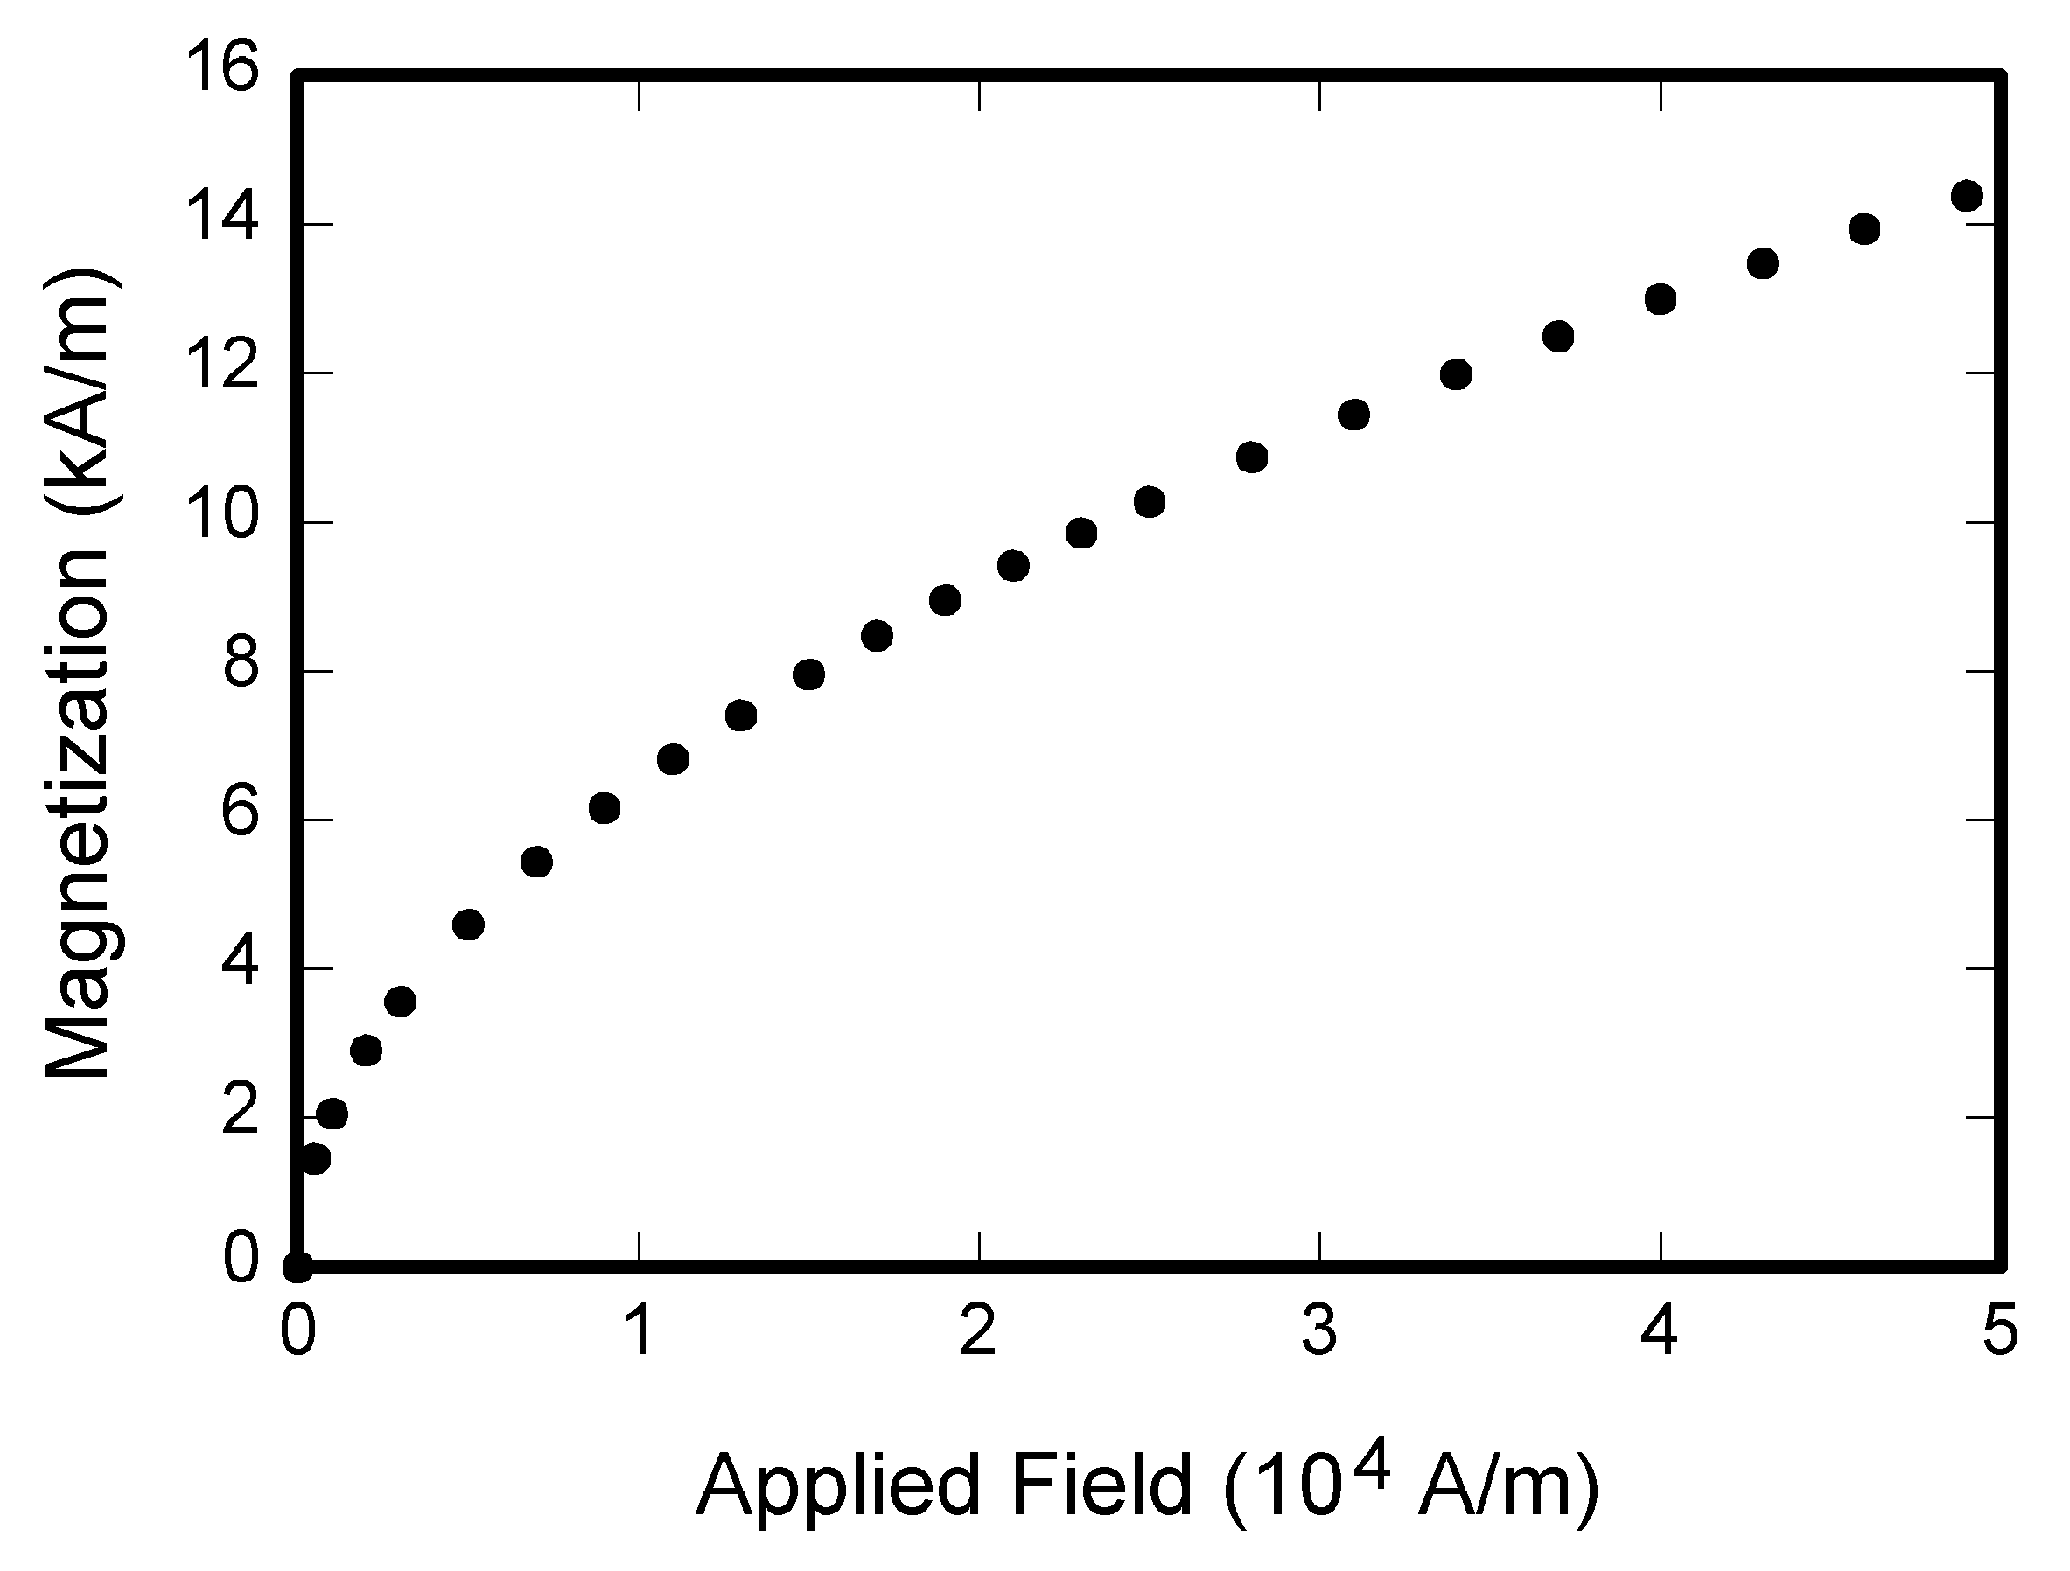
\includegraphics{fig1.png}}
% \caption{Example of a figure caption.}
% \label{fig:qwe}
% \end{figure}

% Figure Labels: Use 8 point Times New Roman for Figure labels. Use words 
% rather than symbols or abbreviations when writing Figure axis labels to 
% avoid confusing the reader. As an example, write the quantity 
% ``Magnetization'', or ``Magnetization, M'', not just ``M''. If including 
% units in the label, present them within parentheses. Do not label axes only 
% with units. In the example, write ``Magnetization (A/m)'' or ``Magnetization 
% \{A[m(1)]\}'', not just ``A/m''. Do not label axes with a ratio of 
% quantities and units. For example, write ``Temperature (K)'', not 
% ``Temperature/K''.

% \section*{Acknowledgment}

% The preferred spelling of the word ``acknowledgment'' in America is without 
% an ``e'' after the ``g''. Avoid the stilted expression ``one of us (R. B. 
% G.) thanks $\ldots$''. Instead, try ``R. B. G. thanks$\ldots$''. Put sponsor 
% acknowledgments in the unnumbered footnote on the first page.

% \section*{References}

% Please number citations consecutively within brackets \cite{b1}. The 
% sentence punctuation follows the bracket \cite{b2}. Refer simply to the reference 
% number, as in \cite{b3}---do not use ``Ref. \cite{b3}'' or ``reference \cite{b3}'' except at 
% the beginning of a sentence: ``Reference \cite{b3} was the first $\ldots$''

% Number footnotes separately in superscripts. Place the actual footnote at 
% the bottom of the column in which it was cited. Do not put footnotes in the 
% abstract or reference list. Use letters for table footnotes.

% Unless there are six authors or more give all authors' names; do not use 
% ``et al.''. Papers that have not been published, even if they have been 
% submitted for publication, should be cited as ``unpublished'' \cite{b4}. Papers 
% that have been accepted for publication should be cited as ``in press'' \cite{b5}. 
% Capitalize only the first word in a paper title, except for proper nouns and 
% element symbols.

% For papers published in translation journals, please give the English 
% citation first, followed by the original foreign-language citation \cite{b6}.

\begin{thebibliography}{00}
\bibitem{ref1} H. Alam et al., “Iot based smart baby monitoring system with emotion recognition using machine learning,” Wireless Communications and Mobile Computing, vol. 2023, no. 1, p. 1175450, 2023.
\bibitem{ref2} Y. Singh, “Iot based baby monitoring system,” International  Journal for Research in Applied Science and Engineering Technology, vol. 9, no. 12, pp. 2184–2190, Dec. 2021, issn: 2321-9653. doi: 10.22214/ijraset.2021.39699. [Online]. Available: http://dx.doi.org/10.22214/ijraset.2021.39699.
\bibitem{ref3} M. M. Hossain et al., “Internet of things in pregnancy care coordination and management: A systematic review,” Sensors, vol. 23, no. 23, p. 9367, Nov. 2023, issn: 1424-8220. doi: 10.3390/s23239367. [Online]. Available: http://dx.doi.org/10.3390/s23239367.
\bibitem{ref4} H. M. Ishtiaq Salehin et al., “Development of an iot based smart baby monitoring system with face recognition,” in 2021 IEEE World AI IoT Congress (AIIoT), 2021, pp. 0292–0296. doi: 10.1109/AIIoT52608.2021.9454187.
\bibitem{ref5} S. Joseph et al., “Iot based baby monitoring system smart cradle,” in 2021 7th International Conference on Advanced Computing and Communication Systems (ICACCS), vol. 1, 2021, pp. 748–751. doi: 10.1109/ICACCS51430.2021.9442022.
\bibitem{ref6} M. R. Kumar et al., “Smart infant baby monitoring system using iot,” International Journal for Research in Applied Science and Engineering Technology, vol. 11, no. 4, pp. 3003 3008, Apr. 2023, issn: 2321-9653. doi: 10.22214/ijraset.2023.50764. [Online]. Available: http://dx.doi.org/10.22214/ijraset.2023.50764.
\bibitem{ref7}  S. Mishra, “Development of rtos based internet connected baby monitoring system,”Indian Journal of Public Health Research Development, vol. 9, no. 2, p. 345, 2018.
\bibitem{ref8} D. T. P. Hapsari et al., “Smart caregiving support cloud integration systems,” in 2024 International Conference on Smart Computing, IoT and Machine Learning (SIML), 2024, pp. 167–173. doi: 10.1109/SIML61815.2024.10578217.
\bibitem{ref9}  F. Akta et al., “Real time infant health monitoring system for hard of hearing parents,” in 2016 Medical Technologies National Congress (TIPTEKNO), IEEE, 2016, pp. 1–4.
% \bibitem{b10} ``Treatment episode data set: discharges (TEDS-D): concatenated, 2006 to 2009.'' U.S. Department of Health and Human Services, Substance Abuse and Mental Health Services Administration, Office of Applied Studies, August, 2013, DOI:10.3886/ICPSR30122.v2
% \bibitem{b11} K. Eves and J. Valasek, ``Adaptive control for singularly perturbed systems examples,'' Code Ocean, Aug. 2023. [Online]. Available: https://codeocean.com/capsule/4989235/tree
\end{thebibliography}

% \vspace{12pt}
% \color{red}
% IEEE conference templates contain guidance text for composing and formatting conference papers. Please ensure that all template text is removed from your conference paper prior to submission to the conference. Failure to remove the template text from your paper may result in your paper not being published.

\end{document}
